\documentclass[aps, pre, onecolumn, a4paper, floatfix]{revtex4}
%\documentclass[twocolumn]{revtex4}
\usepackage{graphicx}
\usepackage{amsmath}
\usepackage{placeins}
\usepackage{color}
\usepackage{hyperref}
%\usepackage{bug}
%\bibliographystyle{plain}




\begin{document}

\title{Message passing problem on random graphs}
\author{Sebastian M.\ Krause}
\affiliation{}
\begin{abstract}

\end{abstract}
%\pacs{89.65.-s, 05.50.+q, 05.65.+b, 64.60.De}
\maketitle

\section*{Question}

Lets assume the generalized configuration model graph ensamble with $N$ nodes, 
where each degree sequences $\{k_i\}$ occurs with probability $\prod_i p_{k_i}$ 
with the degree distribution $p_{k}$. 
(see M.E.J. Newman: Networks, an Introduction; 2010; Eq. (13.30). The generalization 
of the configuration model is important for numerics with small networks, where 
many network realizations are sampled for averiging.) Lets additionally assign to 
every node $i$ a color $c_i\in 1,2,\dots,C$. The color sequence $\{c_i\}$ has 
probability $\prod_i r_{c_i}$ with the color distribution $r_c$. 
How large is the fraction of node pairs, which can be connected via a set of  
paths, such that for every color there exists a path avoiding this color? 

\begin{figure}[htb]
\begin{center}
	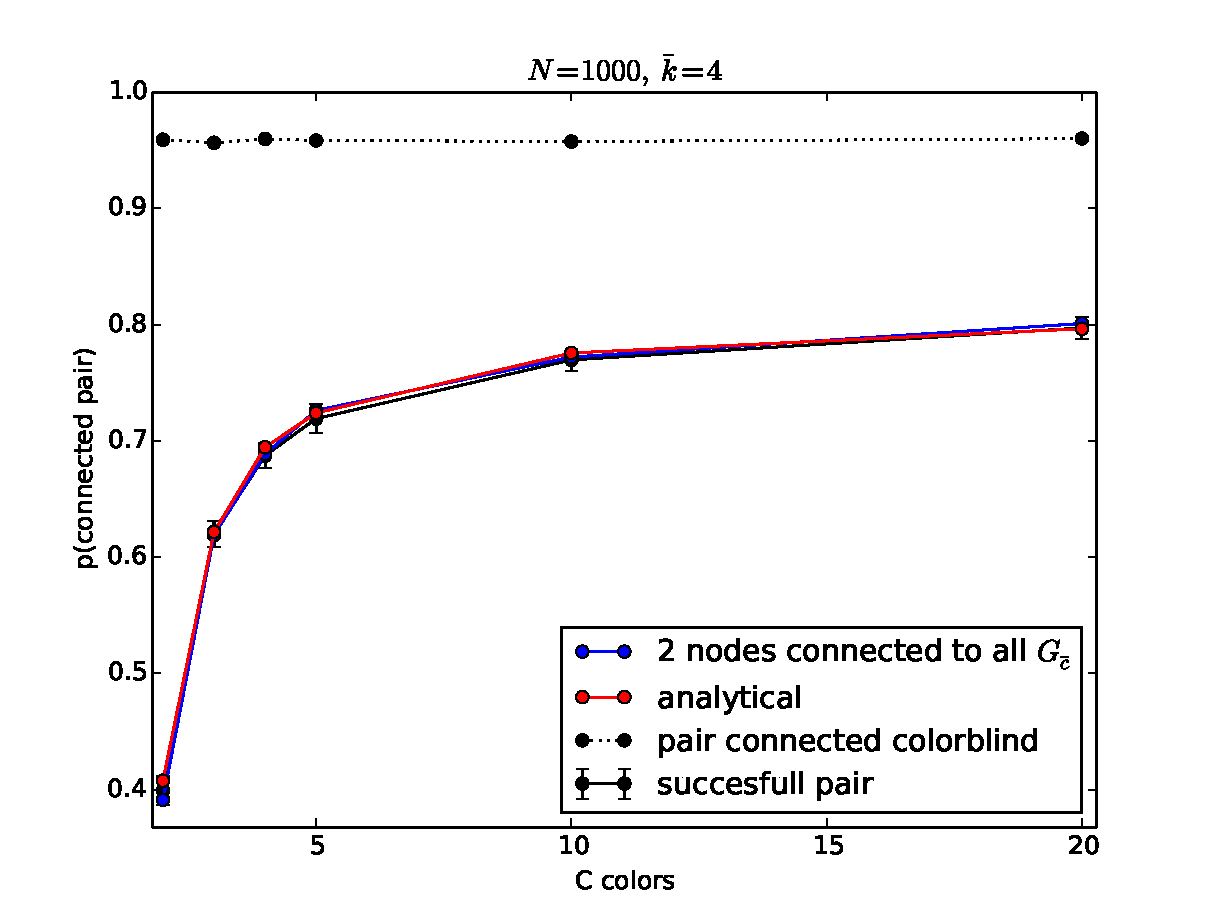
\includegraphics[width=0.6\columnwidth]{finder_C.pdf}
	\caption{}
	\label{fig:model}
\end{center}
\end{figure}
%
For numerical results, we generated Poisson graphs with $N=1000$ (we used the 
Poisson distribution as an approximation to the binomial distribution in 
ER-graphs), and distributed $C$ colors over the nodes, with $r_c=1/C$. 
To check for a single pair, if it can be connected in 
the way as described above, we removed all nodes with the first color (except for 
the node pair under consideration) and 
searched for the shortest path (using a library function returning an empty set, 
if no path exists). Then we took the original graph and removed all nodes with the 
second color etc. If for all colors the shortest path exists, we considered the 
pair as successful. The case of a successful pair with a smaller number of 
paths, where e.g. one path avoids two colors, is included, as such a path could 
just be counted twice with our procedure. We repeated this 200 times with node pairs 
randomly chosen, and calculated the fraction of successful node pairs. See the black 
straight line in figure~\ref{fig:model}, with averages over 50 network realizations. The dotted 
line shows the fraction of node pairs, which are connected with a path which can 
have all colors. 



\section*{Connection to percolation}

For estimating the fraction of successful pairs analytically, results from percolation 
theory can be used. First of all, the existence of a (colorblind) giant component clearly is a 
prerequisite for the existence of a macroscopic fraction of successful node pairs. With the 
generating functions of degree $g_0(z)=\sum_k p_k z^k$ and excess degree 
$g_1(z)=\sum_k q_k z^k$, the size of the giant component $S$ can be calculated (assuming infinite
networks which are locally treelike) using 
the average probability $u$, ``that a vertex is not connected to the giant component 
via its connection to some particular neighboring vertex'' (Newman, page 461): 
\begin{align}
u &= g_1(u)\\
S &= 1 - g_0(u).
\end{align}
Lets call the set of all nodes belonging to the giant component as ${\mathcal G}$. 
Another prerequisite is the existence of a giant component after deleting all nodes of one 
of the colors $c$. Lets call the analogue of $u$ after all nodes of color $c$ are 
deleted as $u_{\bar c}$, the set of all nodes in the remaining giant component as 
${\mathcal G}_{\bar c}$, and its size as $S_{\bar c}$. 
We have 
\begin{align}
\phi_{\bar c} &= 1-r_c\\
u_{\bar c} &= 1-\phi_{\bar c} + \phi_{\bar c} g_1(u_{\bar c})\\
S_{\bar c} &= \phi_{\bar c} (1-g_0(u_{\bar c})).
\end{align}
Finally a node pair is for sure successful, if for both nodes the following 
holds: For every color $c$ there exists at least one neighbor belonging to 
${\mathcal G}_{\bar c}$. Lets call the set of all nodes fulfilling this 
condition as ${\mathcal G}_{\rm color}$, and its size as $S_{\rm color}$. 
The fraction of successful node pairs should be approximately $S_{\rm color}^2$. 

We tested this hypothesis with numerical results. For every color $c$, we labeled all the 
nodes with a boolean variable, if they belong to ${\mathcal G}_{\bar c}$ (more precise, if they 
belong to the largest component, as the networks are finite). A single node can 
belong to different components ${\mathcal G}_{\bar c}$. Then we searched for 
nodes which can be successful in a node pair. For a single node, we iterated over 
all the neighbors and collected all the memberships ${\mathcal G}_{\bar c}$ present. If for 
all colors $c$ there is at least one membership ${\mathcal G}_{\bar c}$ among the neighbors, 
the node belongs to ${\mathcal G}_{\rm color}$ and is
potentially successful in a pair. We calculated the 
fraction $S_{\rm color}$ over all nodes, and by squaring this we got an estimate for 
successful node pairs. This procedure ignores paths in small components, but 
is a good estimate, as can be seen with the blue line in figure~\ref{fig:model}. 
This procedure is much faster as well.


\section*{Analytical results}

As we have tested numerically that $S_{\rm color}$ can be used to describe the success of node 
pairs in connecting over paths with avoided colors, it is useful to assess this quantity 
analytically. We will do this assuming an infinite, locally treelike network. 
We calculate $S_{\rm color}$ as the probability, that a randomly chosen node belongs to 
${\mathcal G}_{\rm color}$. A randomly chosen node has exactly $k$ links with probability $p_k$. We 
need the probability that these links connect to all components ${\mathcal G}_{\bar c}$. As 
${\mathcal G}_{\bar c}$ are subsets of ${\mathcal G}$, only links connecting to ${\mathcal G}$ 
can contribute. We therefore use the conditional probability
%
\begin{align}
Q_{k,k'} &={k \choose k'}(1-u)^{k'}u^{k-k'}
\end{align}
%
that out of $k$ links $k'$ connect to the giant component. Further the distribution of colors 
among the nodes these links connect to is crucial. 
%
\begin{align}
R_{k',\vec \kappa} &=\frac{k'!}{\kappa_1! \times \dots \times \kappa_C!} \,
(r_1)^{\kappa_1} \times \dots \times (r_C)^{\kappa_C}\,
\delta_{k',\kappa_1+\dots + \kappa_C}
\end{align}
%
denotes the conditional probability that out of those $k'$ links $\kappa_1$ connect to nodes of 
color 1, $\kappa_2$ links connect to nodes of color 2 etc. 

Lets now concentrate on one color $c$. We have 
$k'-\kappa_c$ links which potentially can connect to the desired component ${\mathcal G}_{\bar c}$. 
According to the choices we have made so far, those links connect to the giant component 
${\mathcal G}$ and none of the nodes they are connecting to has color $c$. Therefore, a single 
of those links does not connect 
to ${\mathcal G}_{\bar c}$ with the conditional probability 
%
\begin{align}
U_{\bar c} &= 1 - \frac{1-u_{\bar c}}{(1-u)\phi_{\bar c}}.
\end{align}
The last term is the probability, that over a single link a connection to ${\mathcal G}_{\bar c}$
is established, if this link already fulfills the following precondition: 
It connects to ${\mathcal G}$ and at the same time to a node without color $c$. 
This precondition has probability $(1-u)\phi_{\bar c}$, as colors are randomly distributed and therefore 
are not correlated with the probability $u$ or $1-u$. As the links connecting to ${\mathcal G}_{\bar c}$ 
are a subset of all links fulfilling the precondition, the conditional probability can be 
calculated by dividing with the probability of the precondition. 
Notice that the additional information of the explicit color $c'$, instead of only stating that the color 
is not $c$, does not alter the results, as a further restriction of the colors 
would meat the numerator and denominator identically and therefore would cancel out. 

There is at least one link connecting to ${\mathcal G}_{\bar c}$ with probability 
$1-(U_{\bar c})^{k'-\kappa_c}$. The success probabilities for different colors have to be 
multiplied, as all ${\mathcal G}_{\bar c}$ have to be reached at the same time. 
Putting everything together we have 
%
\begin{align}
S_{\rm color} &= \sum_{k=0}^{\infty}p_k \sum_{k'=0}^{k} Q_{k,k'} 
\sum_{\kappa_1,\dots, \kappa_C=0}^{k'} R_{k',\vec \kappa} 
\prod_{c=1}^C [1-(U_{\bar c})^{k'-\kappa_c}],\label{eq:s_color}
\end{align}

esults for Poisson graphs are shown in figure~\ref{fig:model} with the red line, showing 
$S_{\rm color}^2$ as the probability of two nodes to be connected via all Components 
$G_{\bar c}$ simultaneously. Instead of evaluating the sums over $k'$ and $\vec \kappa$ 
in eq.~\ref{eq:s_color}, we sampled 5000 events for every $k$.The outcome compares well with 
numerical results. 

To compare with the standard percolation, we can use $\sum_{k=0}^{\infty}p_k \sum_{k'=0}^{k} Q_{k,k'} 
\sum_{\kappa_1,\dots, \kappa_C=0}^{k'} R_{k',\vec \kappa} = 1$ (total probability is one) together with 
the fact that $\prod_{c=1}^C [1-(U_{\bar c})^{k'-\kappa_c}]=0$ whenever $k'<2$ (at least for one 
color then $k'-\kappa_c=0$). Therefore we have 
%
\begin{align}
S_{\rm color} &< 1-\sum_{k=0}^{\infty}p_k [u^k +k (1-u) u^{k-1}]\\
 &= 1 - g_0(u) - (1-u) \left.\frac{{\rm d}g_0(z)}{{\rm d}z}\right|_{z=u}\\
 &= S_{{\rm color},\infty}.
\end{align}
%
The upper limit $S_{{\rm color},\infty}$ for $S_{\rm color}$ reflects the fact, that every node has to be 
connected to the giant component at least over two links. It therefore includes a reduction 
compared to the standard percolation result $1-g_0(u)$. In the limit of many colors and small 
probabilities $r_c$, $S_{\rm color}$ can come close to $S_{{\rm color},\infty}$, as in this case $U_{\bar c}$ comes 
close to zero and only nodes fail which have less than two links connecting to the giant component.  


\section*{Phase transition for Poisson graphs}

\begin{figure}[htb]
\begin{center}
	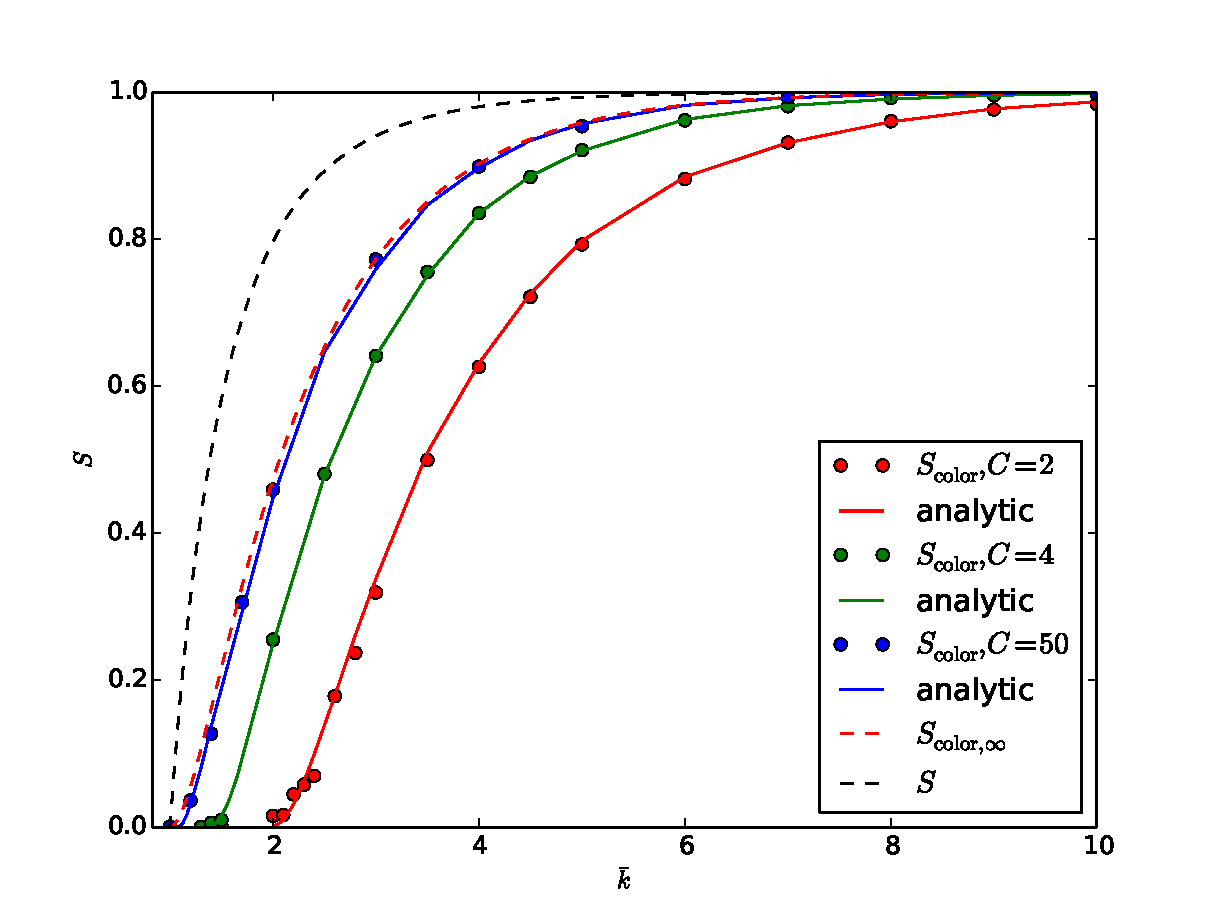
\includegraphics[width=0.52\columnwidth]{S_color_k.pdf}
	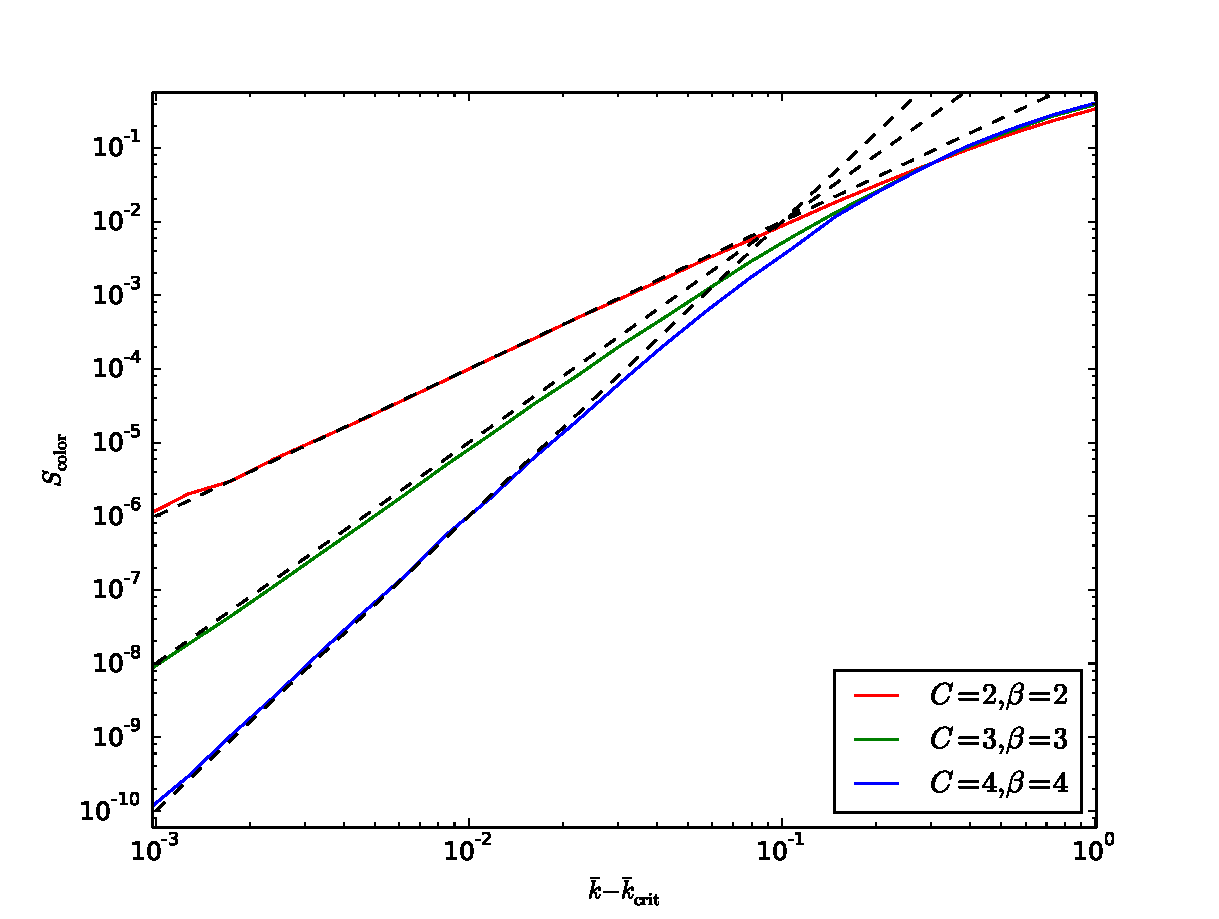
\includegraphics[width=0.47\columnwidth]{S_color_k_beta.pdf}
	\caption{}
	\label{fig:pt}
\end{center}
\end{figure}

In figure~\ref{fig:pt} on the left, the dependence of $S_{\rm color}$ on the average degree is shown for different numbers 
of colors $C$ ($r_c=1/C$). Comparing to the standard giant component size $S$ (dashed black line in the figure), 
the percolation sets in at increasing $\bar k$ with smaller numbers of colors, and the component size grows 
slower to the saturation value of one. The circles show numerical results with $N=1000$ and 10 network realizations, 
the lines show results of equation~\ref{eq:s_color}, both correspond well. $S_{\rm color}$ comes close to 
$S_{{\rm color},\infty}$ (shown with dashed red line) already for $C=50$. We see that $S_{{\rm color},\infty}$ 
is remarkably reduced compared to $S$ for small $k$, but has the same critical parameter. 
For the Poisson graph we have $S_{\rm color,\infty}=S-{\bar k} S (1-S)$, and for small positive ${\bar k}-1$ 
the giant component grows approximately with $S\approx 2 ({\bar k}-1)/{\bar k}^2$. Therefore
\begin{align}
S_{\rm color,\infty}\approx 2({\bar k}-1)^2/\bar k,
\end{align}
which grows slowly for small parameter ${\bar k}-1$. 

To find the critical ${\bar k}_{\rm crit}$ and the critical exponent $\beta$ with 
$S_{\rm color}\propto ({\bar k}-{\bar k}_{\rm crit})^{\beta}$, we expand equation~\ref{eq:s_color} for $U_{\bar c}$ 
close to one with $U_{\bar c}=1-\varepsilon$. We have ${\bar k}_{\rm crit}=C/(C-1)$, as for values larger 
than this $U_{\bar c}$ falls below one. The expansion gives us leading terms 
$S_{\rm color}\propto \varepsilon^C \propto({\bar k}-{\bar k}_{\rm crit})^C$, therefore $\beta=C$. This is tested 
for $C=2,3,4$, as shown in figure~\ref{fig:pt} on the right. Numerical testing would need very large networks. 



\section*{Heterogeneous color distribution}

With heterogeneous color distributions, the color with the largest probability $r_c$ dominates 
the behavior, as it corresponds to the largest $U_{\bar c}$. For Poisson graphs, $U_{\bar c}$ 
falls below one at ${\bar k}=1/(1-r_c)$, and as long as one $U_{\bar c}$ is one, equation~\ref{eq:s_color}
gives zero. We have ${\bar k}_{\rm crit}=1/(1-\max_c r_c)$. With the expansion according to 
$U_{\bar c}=1-\varepsilon$ as described above, 
the critical exponent $\beta$ is given by the degeneration of the largest color frequency. Critical 
parameter and critical exponent have been tested with Poisson network realizations of size $N=1000$ 
with some special color distributions up to $C=7$ colors with non- and single-degenerated 
largest color frequency (results not shown). However, the 
behavior of systems with non-degenerated but close highest frequencies has to be analyzed. 



\section*{Broad degree distribution}

In figure~\ref{fig:broad}, results for graphs with broad degree distributions with 
$p_k=n k^{-\alpha}$ are shown. $n$ is a normalization constant, and the giant component 
exists between $\alpha=2$ and $\alpha=3.5$. We see a strong reduction of 
$S_{{\rm color},\infty}$ compared to $S$, while the number of colors ($r_c=1/C$) plays 
a minor role. Numerical results are averages over 50 networks of size $N=10\,000$. 
For evaluating equation~\ref{eq:s_color}, 1000 events where sampled for every $k$. 


\begin{figure}[htb]
\begin{center}
	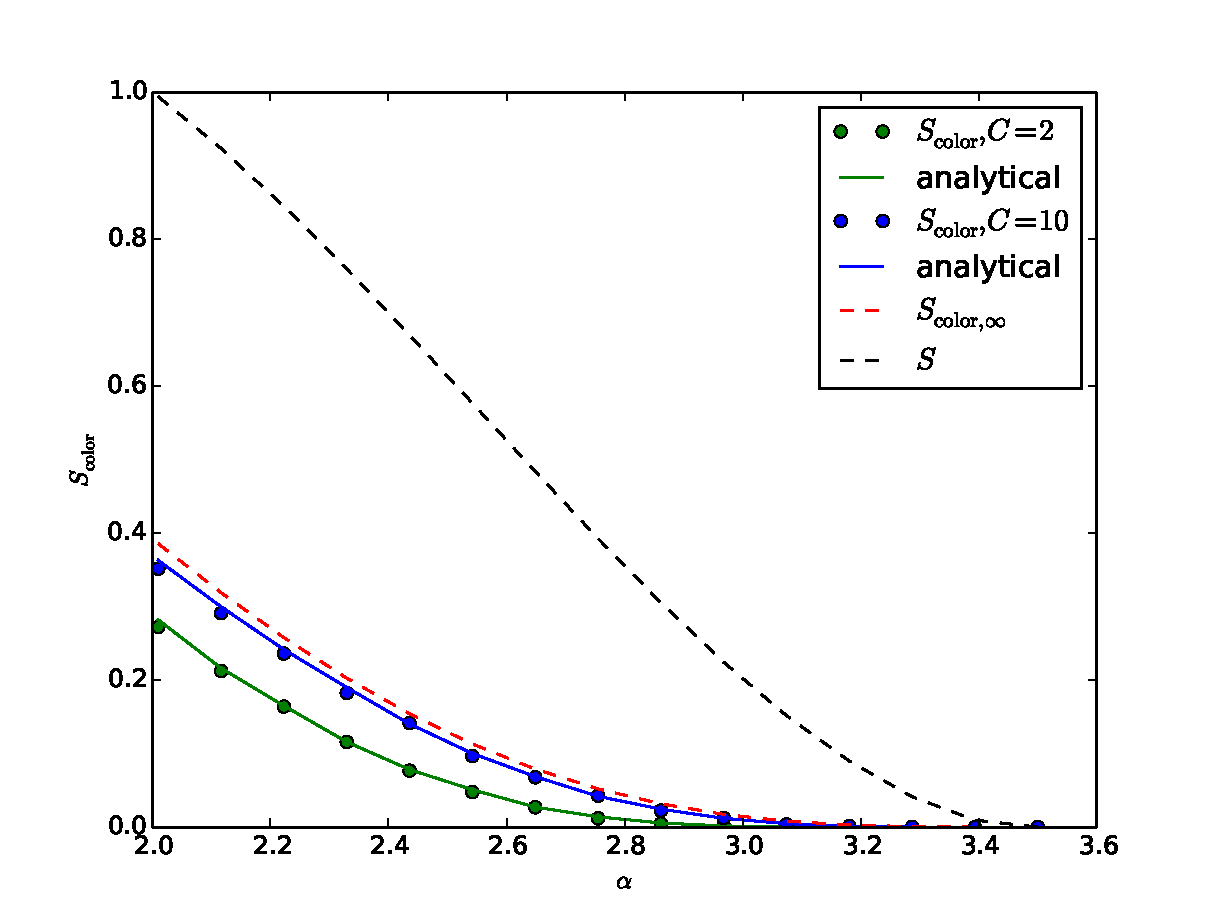
\includegraphics[width=0.6\columnwidth]{S_color_broad.pdf}
	\caption{}
	\label{fig:broad}
\end{center}
\end{figure}





\section*{Appendix: Independence of components for Poisson graphs}

In equation~\ref{eq:s_color}, the probabilities $1-U_{\bar c}^{k'-k_c}$ for 
different colors may show dependencies 
among each other limiting the usability of the equation. In the following we 
discuss one particular case for Poisson graphs, in order to illustrate a sort 
of independence. Lets assume we only have one link connecting to a node in the 
giant component, and the node has color 3. Can the probability, that this link connects 
to ${\mathcal G}_{\bar 1}$ and ${\mathcal G}_{\bar 2}$ at the same time 
really be written as the product $(1-U_{\bar 1})(1-U_{\bar 2})$? 
As for Poisson graphs we 
have $S=1-u$, instead of discussing link probabilities $u$ we can concentrate on 
node probabilities $S$. 

We use the notation $S\left({\mathcal Y}\middle|{\mathcal X}\right)$ to denote 
the fraction of nodes in a set ${\mathcal Y}$ which is a subset of ${\mathcal X}$. With 
the set ${\mathcal N}$ of all nodes in the network we have 
$S_{\bar c}=S\left({\mathcal G}_{\bar c}\middle|{\mathcal N}\right)$. Clearly they must 
be dependent, as 
$S\left({\mathcal G}_{\bar 1}\cap {\mathcal G}_{\bar 2}\cap \dots 
\cap {\mathcal G}_{\bar C}\middle| {\mathcal N}\right)=0\neq 
S\left({\mathcal G}_{\bar 1}\middle| {\mathcal N}\right)\times\dots \times 
S\left({\mathcal G}_{\bar C}\middle| {\mathcal N}\right)$. 
Lets call the set of all nodes with color c as ${\mathcal A}_c$, 
and the set of all nodes without this color as ${\mathcal A}_{\bar c}$. 

Back to our case with the Poisson graph, we have for $c=1,2$
\begin{align}
1-U_{\bar c} &=\frac{S_{\bar c}}{S (1-r_c)}\\
 &= S\left({\mathcal G}_{\bar c} \cap {\mathcal A}_{\bar c} \middle| {\mathcal G} \cap {\mathcal A}_{\bar c} \right)\\
 &= S\left({\mathcal G}_{\bar c} \cap {\mathcal A}_{3} \middle| {\mathcal G} \cap {\mathcal A}_{3} \right).
\end{align}
The last equation is intuitive, as the coloring of nodes is random, and it was tested numerically (results not shown). 
In order to test if the product $(1-U_{\bar 1})(1-U_{\bar 2})$ reflects the probability of 
connecting to ${\mathcal G}_{\bar 1}$ and ${\mathcal G}_{\bar 2}$ at the same time, 
we have to check if 
\begin{align}
S\left({\mathcal G}_{\bar 1}\cap {\mathcal G}_{\bar 2} \cap {\mathcal A}_3 \middle| {\mathcal G} \cap {\mathcal A}_3 \right)=
S\left({\mathcal G}_{\bar 1} \cap {\mathcal A}_3 \middle| {\mathcal G} \cap {\mathcal A}_3 \right)\times 
S\left({\mathcal G}_{\bar 2} \cap {\mathcal A}_3 \middle| {\mathcal G} \cap {\mathcal A}_3 \right)
\end{align}
holds. The comparison of the left hand side and the right hand side 
is shown in figure~\ref{fig:corr} for networks with $N=1000$. For every number of colors $C=3,4,5,10$, 
ten network realizations were used. So we have tested numerically, that 
equation~\ref{eq:s_color} is useful at least in this very simple case. This was 
to illustrate a sort of independence of the conditional probabilities for connecting 
to color-avoiding giant components. The generalization to many links and 
general degree distributions is missing so far. 



\begin{figure}[htb]
\begin{center}
	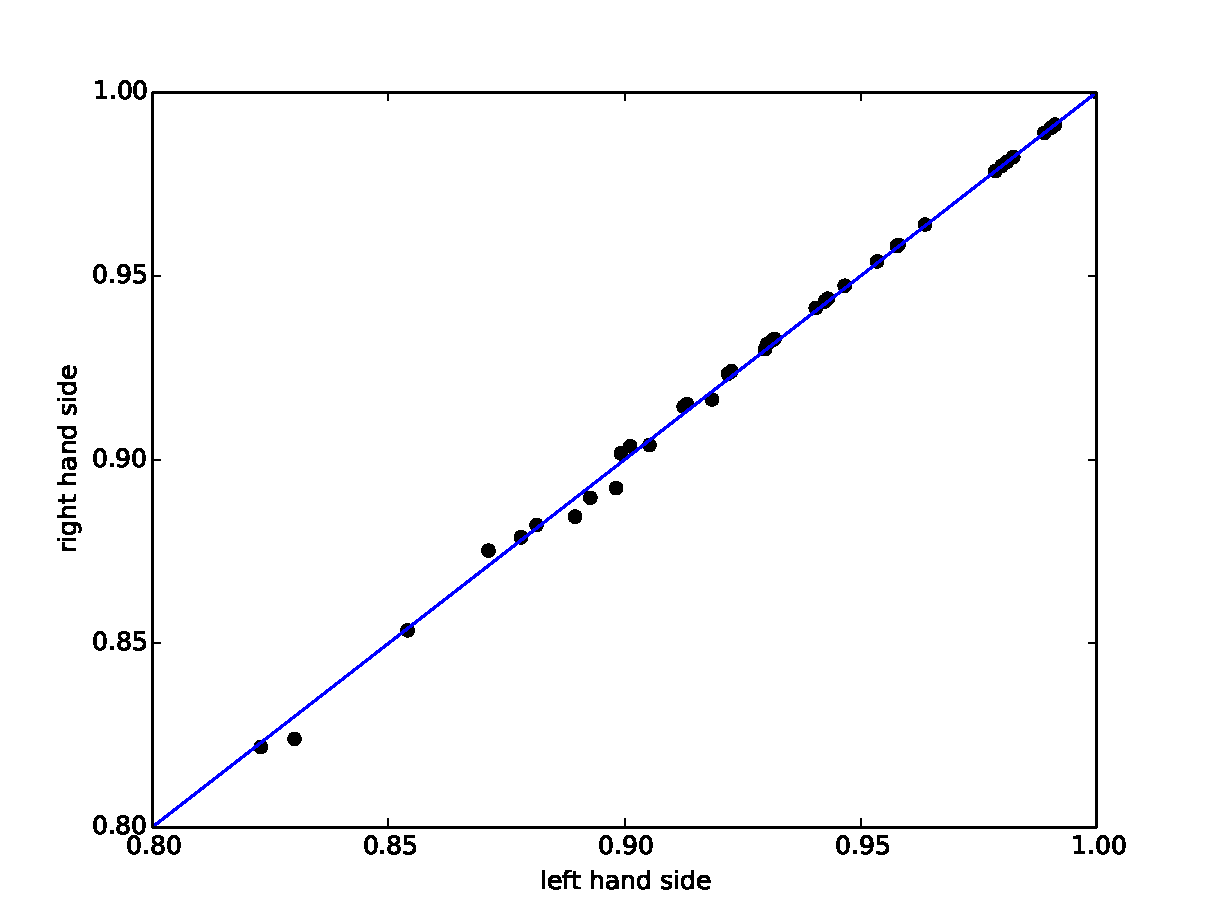
\includegraphics[width=0.6\columnwidth]{finder_C_correlated.pdf}
	\caption{}
	\label{fig:corr}
\end{center}
\end{figure}




\end{document}
